\documentclass[]{article}

\usepackage{graphicx}
\usepackage{subcaption}

%opening
\title{ APP TITLE? \\
	\begin{large} 
		Design and Implementation of Mobile Application Project
	\end{large}}

\author{Antonio Ercolani - 10621728\\Riccardo Nannini - 10626268}
\date{Prof Luciano Baresi - Anno Accademico 2020/2021}


\begin{document}
	
	\maketitle
	
	\begin{paragraph}
		\newline
	\end{paragraph}
	
	\tableofcontents
	
	\newpage
	
	\section{Main goal}
	
	Help apartment mates to deal with the daily domestic problems such as payments, failures, timetables etc...
	
	\section{Application functions}
	
		\subsection{Basic functionality}
		\begin{itemize}
			\item Payment manager
			\item Failures report 
			\item Organize custom timetables
			\item Indicate anything on a "master" apartment calendar 
			\item Missing stuff
		\end{itemize}

		\subsection{Application functions}
		
		\begin{itemize}
			\item Report the apartment presence periods 
			\item Ask for an apartment zone to remain empty for a certain period 
		\end{itemize}

	\section{User interface}
	
	\begin{itemize}
		\item Login/sign up screen
		\item Join/create apartment screen
		\item Main screen with "tab" navigation. 
		\\Tab screens: 
		\begin{itemize}
			\item List of all the notifications (chronologically ordered) 
			, differently labeled according to the type 
			- divided in "active" and "archived"
			\item "New Action" screen in which you can choose between the different actions
			\begin{itemize}
				\item Here there will be a specific screen depends on the action 
			\end{itemize} 
			\item Master calendar
			\item Profile screen
		\end{itemize}
			
	\end{itemize}

	\section{Mockups}
	\begin{figure}[h!]
		\centering
		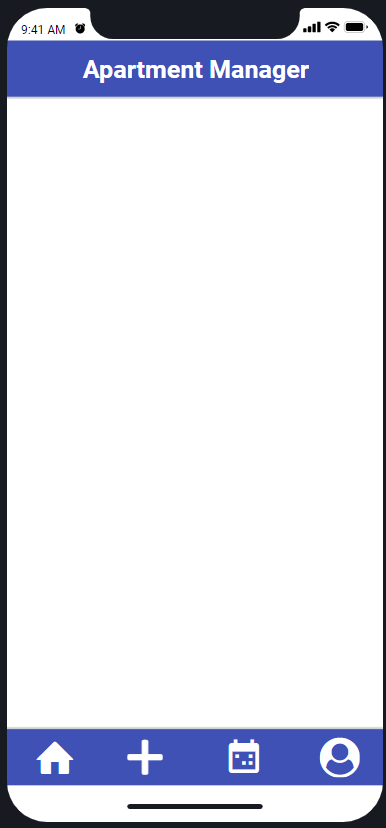
\includegraphics[width=4.5cm]{screen1.png}
		\caption{Main screen mockup}
		\label{fig:boat1}
	\end{figure}

\end{document}
